\documentclass[12pt]{article}
\setcounter{secnumdepth}{0}
\usepackage[english,greek]{babel}
\usepackage[utf8]{inputenc}
\usepackage{enumitem}
\usepackage{titling}
\usepackage{amsmath}
\usepackage{graphicx}
\usepackage{pgfplots}
\setlength{\droptitle}{-12em}

% nemanja's packages and commands
\usepackage{listings}
\lstset{
  basicstyle=\ttfamily,
  mathescape
}
\newcommand\tab[1][1cm]{\hspace*{#1}}
\usepackage{hyperref}

\title{{Ανάλυση Σχεδίαση Συστημάτων Λογισμικού} \\
\vspace{2cm}
{\Huge Εργασία 2017-2018} \\
\vspace{2cm}
{Νέμανια Νέντις}\\
{Α.Μ. 1115201400124}\\
{Κωνσταντίνος Στεφανίδης - Βοζίκης}\\
{Α.Μ. 1115201400192}}


\date{}

\begin{document}
\maketitle
\newpage
\tableofcontents
\newpage

\section{Διαδικαστικά}
Η εργασία αναπτύχθηκε από ομάδα 2 ατόμων.\\
\tab Η δουλειά μοιράστηκε ως εξής:\\ 
\tab Το πρώτο μέλος ασχολήθηκε κυρίως με τα μέρη Β και Γ καθώς και με το τελευταίο ερώτημα του μέρους Α. Το άλλο μέλος ασχολήθηκε κυρίως με τα ερωτήματα 1 εως 8 
του μέρους Α.\\
\tab Κάθε μέλος συμμετείχε στην συζήτηση και βοηθούσε στην διεκπαιρέωση των καθηκόντων του αλλου μέλλους. Είτε αυτό αφορούσε την επαλήθευση της ορθότητάς τους, είτε την ανταλλαγή γνώσεων του θεωριτικού υπόβαθρου.\\
\tab Η συνεργασία έγινε εξ αποστάσεως μέσω Ιστοσελιδων Κοινωνικης Δικτυωσης για τα άμεσα μηνύματα και έπειτα μέσω \textlatin{Skype} για περαιτέρω ανάλυση των προβλημάτων.\\
\tab Ο μεγαλύτερος σύμμαχος στην διαδικασία διαμοιρασμού και οργάνωσης της εργασίας αποτέλεσε η πλατφόρμα διαμοιρασμού και ελέγχου εκδόσεων \href{https://github.com/}{\textlatin{Github}}.\\
\tab Προβλήματα που συναντήσαμε, τα οποία ξεπεράστηκαν εύκολα ήταν:\\
\tab\tab -Η επικοινωνια εξ αποστασεως Ελλαδα-Γαλλια\\
\tab\tab (το ενα μελος ειναι απεσταλμενος στο Ερ.Κεντρο \href{https://www.inria.fr/en/}{\textlatin{Inria}})\\
\tab\tab -Προβλάματα με την Ελληνική υποδομή παροχής \textlatin{internet}.\\
\tab\tab Με αποτέλεσμα το ένα μέλος να πορεύεται με πακέτα δεδομένων\\ \tab\tab κινητής.\\
\tab Η ανάπτυξη διαγραμμάτων έγινε με την βοήθεια εργαλείων \textlatin{StarUML, Visio, draw.io}.\\
\tab Η σύνταξη του τελικού κειμένου έγινε από κοινού μέσω \textlatin{Texmaker LaTeX editor}.


\newpage
\section{Αντικειμενοστραφής Ανάλυση και Σχεδιασμός}
\begin{enumerate}
\item
Οι μη λειτουργικές απαιτήσεις του συστήματος είναι:
\begin{itemize}
\item
Λήψη αντιγράφων (\textlatin{back up}) κάθε ώρα
\item
Λειτουργία του συστήματος 24 ώρες το 24ώρο
\end{itemize}
\item
\begin{tabular}{|l|l|}
\hline
'Εννοια & Περιγραφή \\
\hline
Διδάσκων & Υπάλληλος του πανεπιστημίου που διδάσκει \\
\hline
ΕΔΙΠ & Διδάσκων πλήρους απασχόλησης \\
\hline
Συμβασιούχος & Διδάσκων με σύμβαση συγκεκριμένου χρόνου \\
\hline
Συμβόλαιο & Συμφωνία μεταξύ του πανεπιστημίου και ενός συμβασιούχου \\
\hline
Άδεια & Χρονικό διάστημα που ένας μόνιμος διδάσκων δεν δουλέυει \\ 
\hline
Τρόπος πληρωμής & Τρόπος με τον οποίο ένας διδάσκων λαμβάνει την αμοιβή \\ 
& του από το πανεπιστήμιο \\
\hline
Ειδοποίηση πληρωμής & Τρόπος με τον οποίο ένας συμβασιούχος ενημερώνεται για \\
 & τα χρήματα που εισπράττει από το πανεπιστήμιο \\
\hline
Πληρωμή & Αμοιβή του πανεπιστημίου προς έναν διδάσκοντα για \\ 
& την εργασία του \\ 
\hline
Χρονοκάρτα & Κατάσταση στην οποία ένας συμβασιούχος διδάσκων \\
 & υποβάλλει στο σύστημα για να μετρηθούν οι μέρες \\
 &  και ώρες διδασκαλίας του. \\
\hline
\end{tabular}

\newpage
\item
Το διάγραμμα περιπτώσεων χρήσης είναι το παρακάτω:
\begin{center}
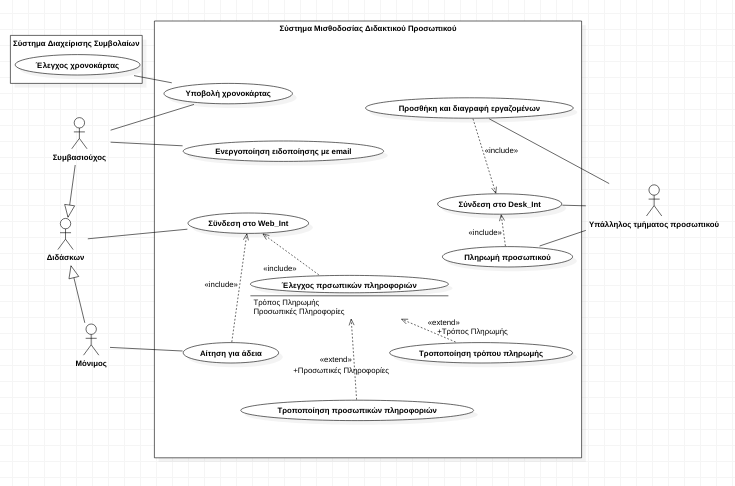
\includegraphics[scale=0.6]{use_case}
\end{center}

\newpage
\item
Το διάγραμμα κλάσεων είναι το παρακάτω:
\begin{center}
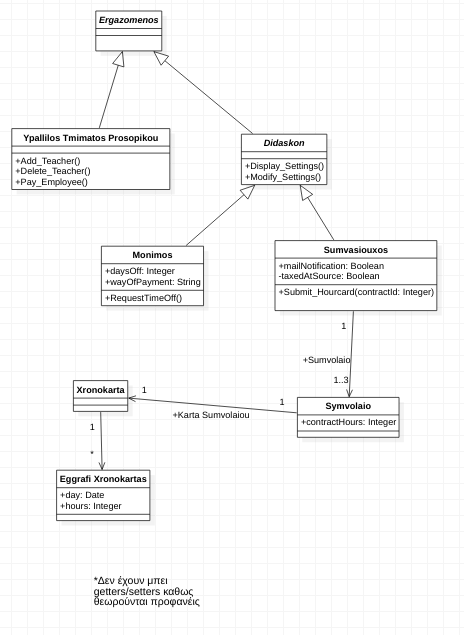
\includegraphics[scale=0.8]{class_diag}
\end{center}

\newpage
\item
\subsection*{Κύριο σενάριο επιτυχίας}
\begin{enumerate}[label=\arabic*.]
\item
Ο χρήστης ανοίγει το \textlatin{Web\_Int}
\item
Ο χρήστης δίνει τα στοιχεία για να κάνει \textlatin{login}
\item
To σύστημα επιβεβαιώνει τα στοιχεία του χρήστη.
\item
To σύστημα εμφανίζει την αρχική σελίδα του \textlatin{Web\_Int} στον χρήστη.
\item
Ο χρήστης διαλέγει την επιλογή "Τροποποίηση τρόπου πληρωμής" 
από το \textlatin{Web\_Int}.
\item
Το σύστημα εμφανίζει την σελίδα με τις επιλογές για τον τρόπο 
πληρωμής στην χρήστη.
\item
Ο χρήστης διαλέγει τον εναλλακτικό τρόπο πληρωμής που επιθυμεί.
\item
Το σύστημα εμφανίζει μήνυμα επιτυχίας αλλαγής τρόπου πληρωμής 
στον χρήστη.
\item
Ο χρήστης κάνει \textlatin{logout} από το σύστημα.
\end{enumerate}

\subsection*{Επεκτάσεις}
3α το σύστημα δεν επιβεβαιώνει τα στοιχεία.
\begin{enumerate}[label=\arabic*.]
\item
Το σύστημα εμφανίζει μήνυμα λάθους και ζητά από τον 
χρήστη να ξαναεισάγει τα στοιχεία του.
\item 
Ο χρήστης πληκτρολογεί ξανά τα στοιχεία του.
\end{enumerate}

\newpage
\item
Το διάγραμμα δραστηριοτήτων για τη διαδικασία χορήγηση άδειας είναι το παρακάτω:
\begin{center}
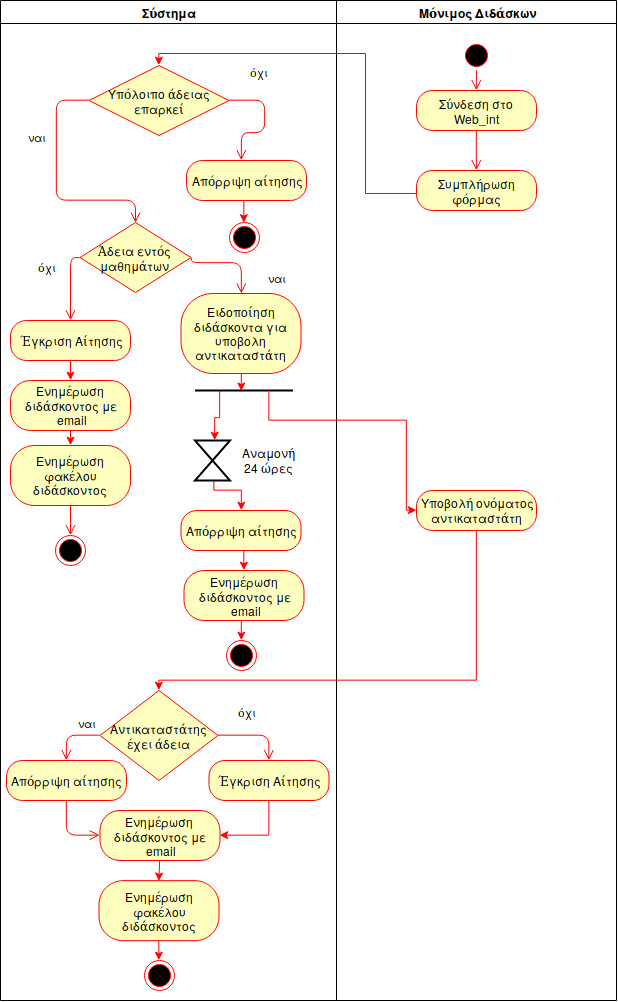
\includegraphics[scale=0.5]{activity}
\end{center}

\newpage
\item
Το διάγραμμα καταστάσεων για το αντικείμενο «Αίτηση Άδειας» είναι το παρακάτω:
\begin{center}
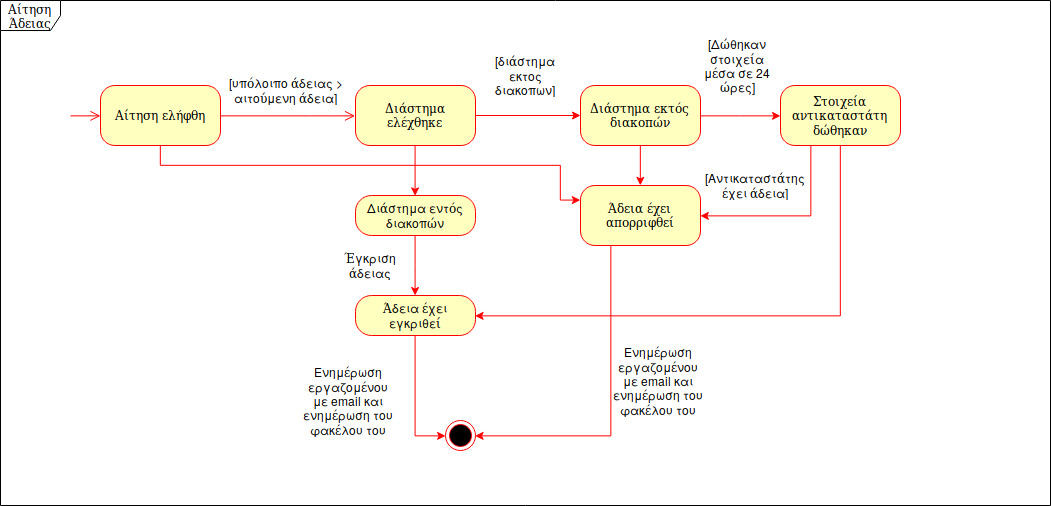
\includegraphics[scale=0.35]{state_diag}
\end{center}

\item
Το διάγραμμα ακολουθίας για την διαδικασία πληρωμής είναι το παρακάτω:
\begin{center}
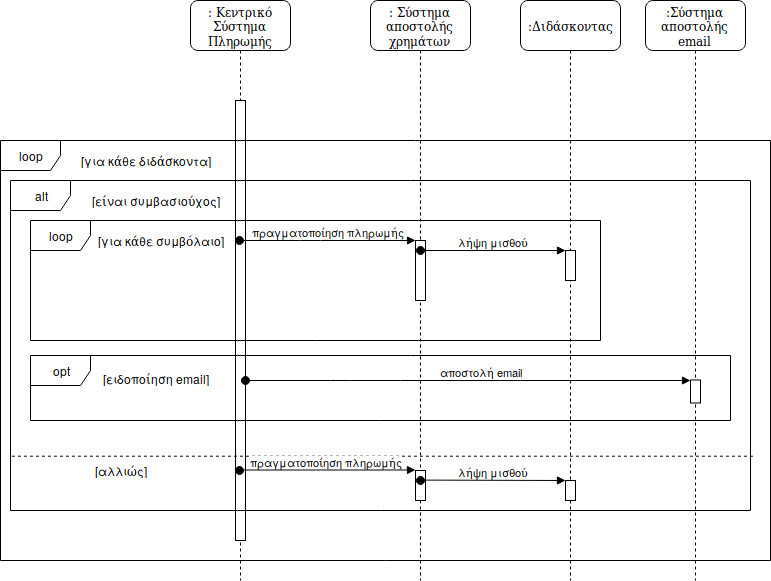
\includegraphics[scale=0.45]{sequence}
\end{center}
\tab Παρατήρηση: Υποθέτουμε οτι το σύστημα πληρωμής χρησιμοποιεί κάποιο 
σύστημα αποστολής χρημάτων (τραπεζικό) καθώς και οτι η 
διαδικασία περιλαμβάνει και την λήψη του μισθού από τον υπάλληλο.

\item
Το διάγραμμα συνεργασιας \textlatin{(collaboration diagram)} ή αλλιως διάγραμα επικοινωνίας \textlatin{(communication diagram)}, όπως πλέον λέγεται στην \textlatin{UML 2} είναι το παρακάτω:
\begin{center}
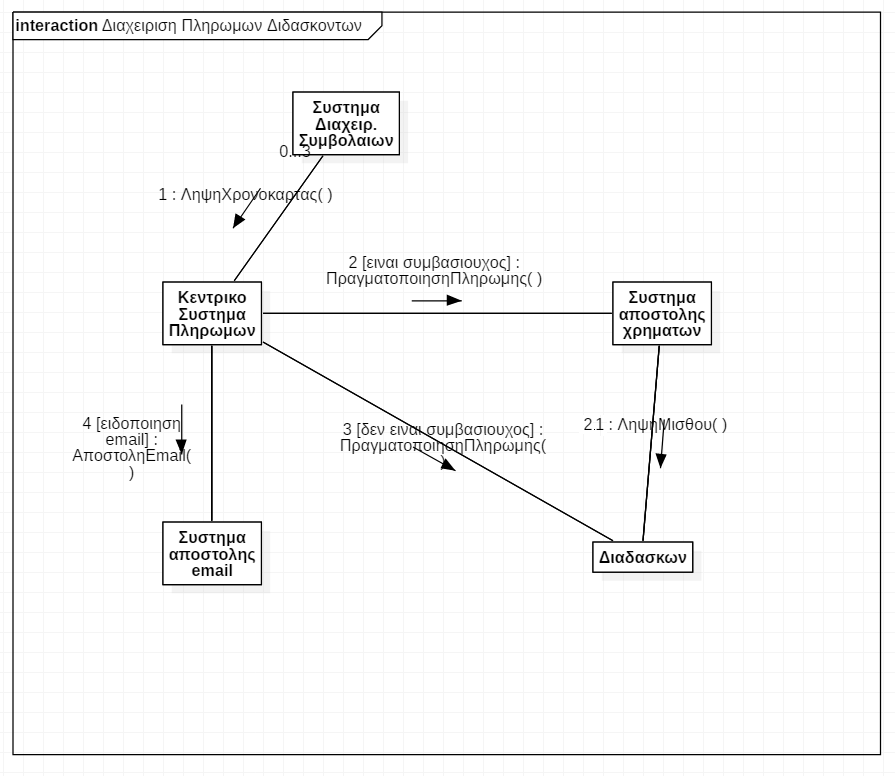
\includegraphics[scale=0.7]{comm_diag}
\end{center}
\end{enumerate}

\newpage
\section{Δομημένη Ανάλυση}
Παρατηρήσεις και παραδοχές εκφώνησης:\\
$\bullet$Αναλύουμε την διαδ. εφαρμογή \textlatin{LAPTOP\_SERVICE} η οποία είναι μέρος του συστήματος Κέντρου Επισκευών. Εστιάζουμε μόνο στην εφαρμογή.\\
$\bullet$Δεν γίνεται διάκριση μεταξύ Τεχνικού που παραλαμβάνει και εισάγει τα στοιχεία της συσκευής και εκεινού που την επισκευάζει. Ουτε είναι απαραίτητο.\\
$\bullet$Δεν έχει ληφθεί υποψήν η διαδικασία της επισκευής, καθώς δεν αφορά την εφαρμογή. Οπότε σε πραγματικό σενάριο ίσως να είχαμε επιπλέον ροές απο την εφαρμογή προς διαδικασίες που αφορούν την επισκευή.\\
$\bullet$Με επιφύλαξη η ροή προς $DIAGNOSE$ από την εφαρμογή καθώς δεν διευκρινίζεται από την εκφώνηση η χρησιμότητα της.

\begin{center}
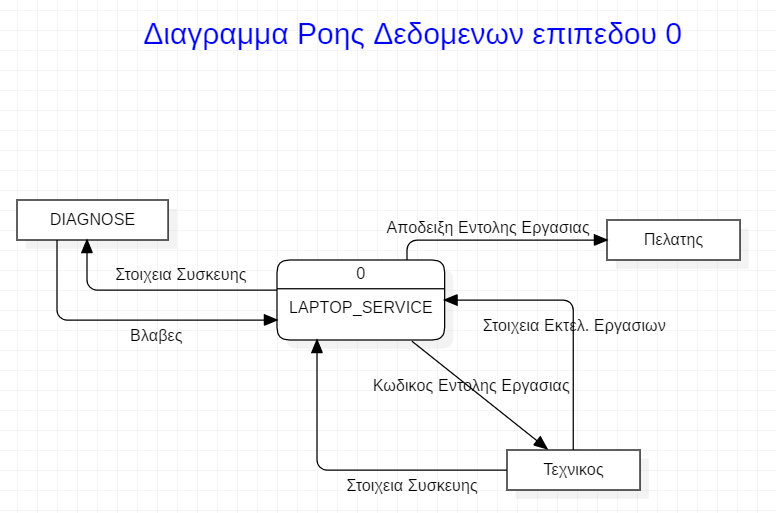
\includegraphics[scale=0.9]{MerosB/B1}
\end{center}
\begin{center}
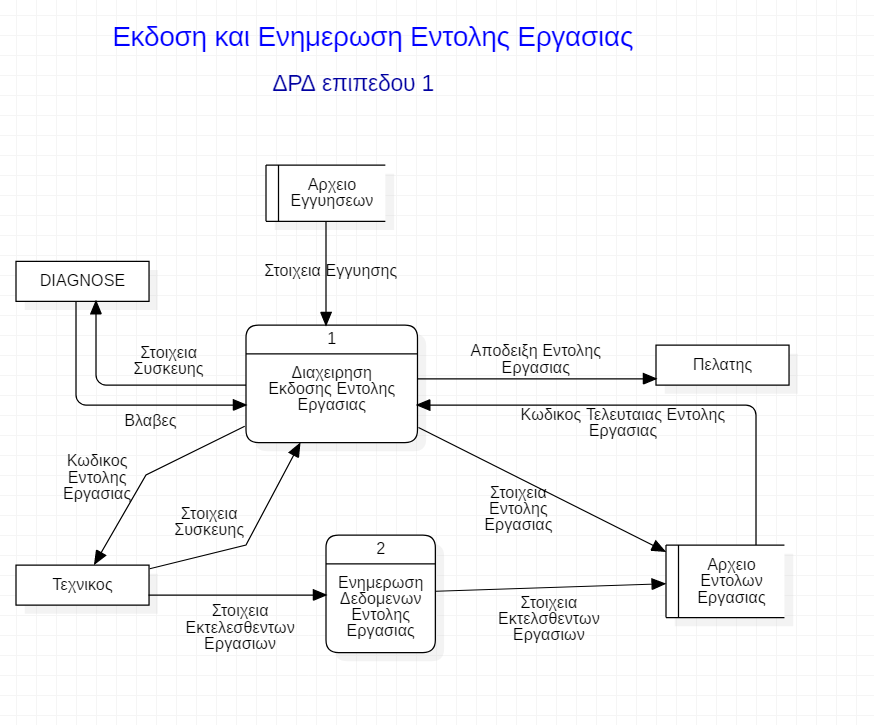
\includegraphics[scale=0.9]{MerosB/B2}
\end{center}
\begin{center}
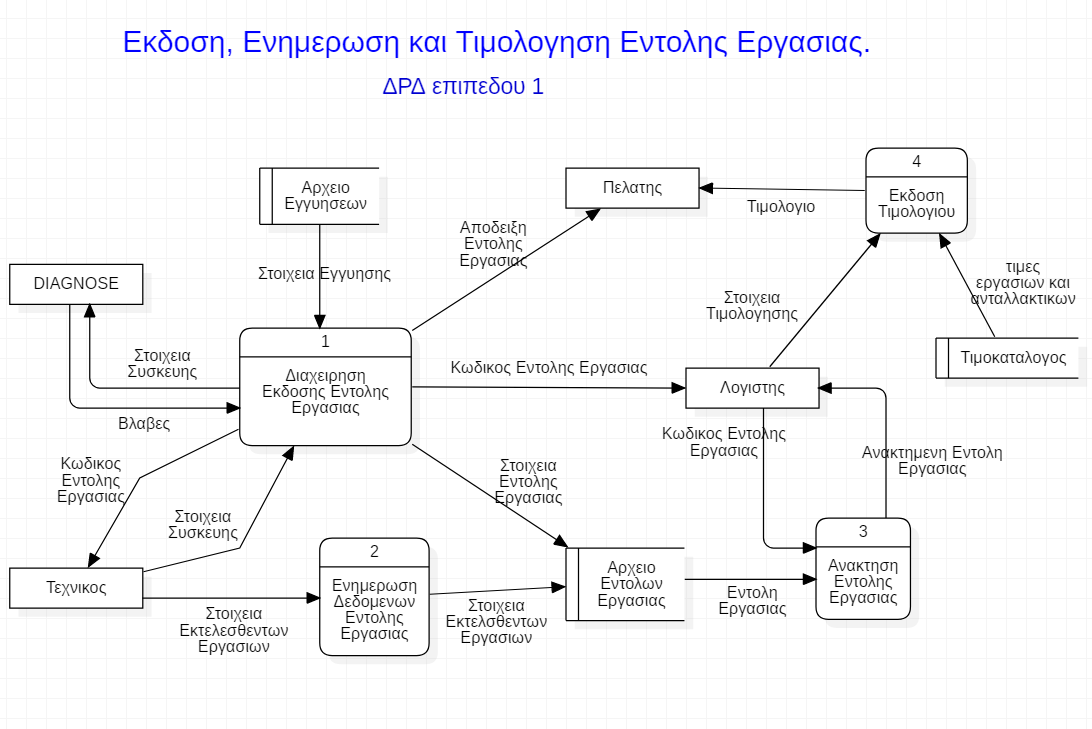
\includegraphics[scale=0.7]{MerosB/B3}
\end{center}
\begin{center}
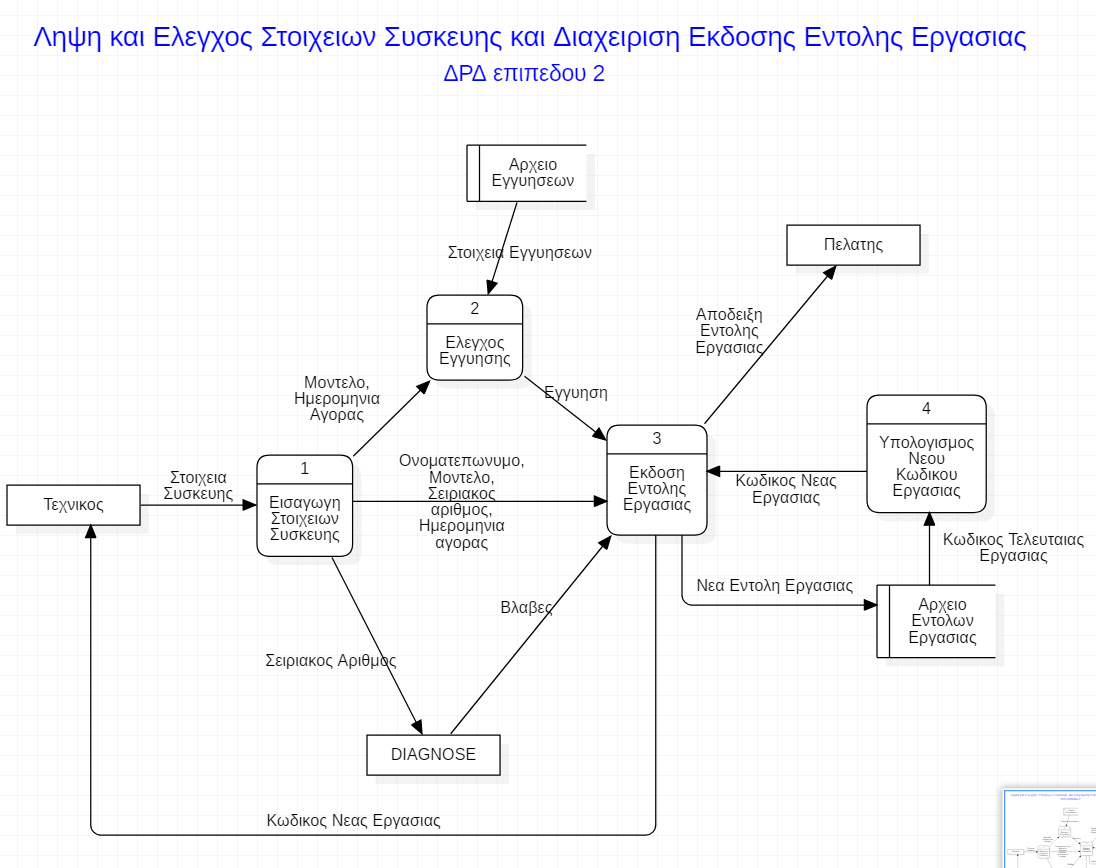
\includegraphics[scale=0.7]{MerosB/B4}
\end{center}

\newpage
\section{Δομημένος Σχεδιασμός}
\begin{enumerate}

\item
\tab Ως κεντρικό μετασχηματισμό επιλέγουμε τον $P1$, καθώς ο $P1$ 
δέχεται δεδομένα εισόδου και εκείνος επενεργεί σε αυτά προκειμένου να δημιουργηθούν δεδομένα εξόδου.\\
\tab Παρατήρηση: Αν θέλαμε να επιλέξουμε Κέντρο Δοσοληψιών ο κατάλληλος μετασχηματισμός θα ήταν ο $P3$.

\begin{center}
\begin{tabular}{c}
Το Διάγραμμα Δομάς Προγράμματος (ΔΔΠ) ειναι:\\
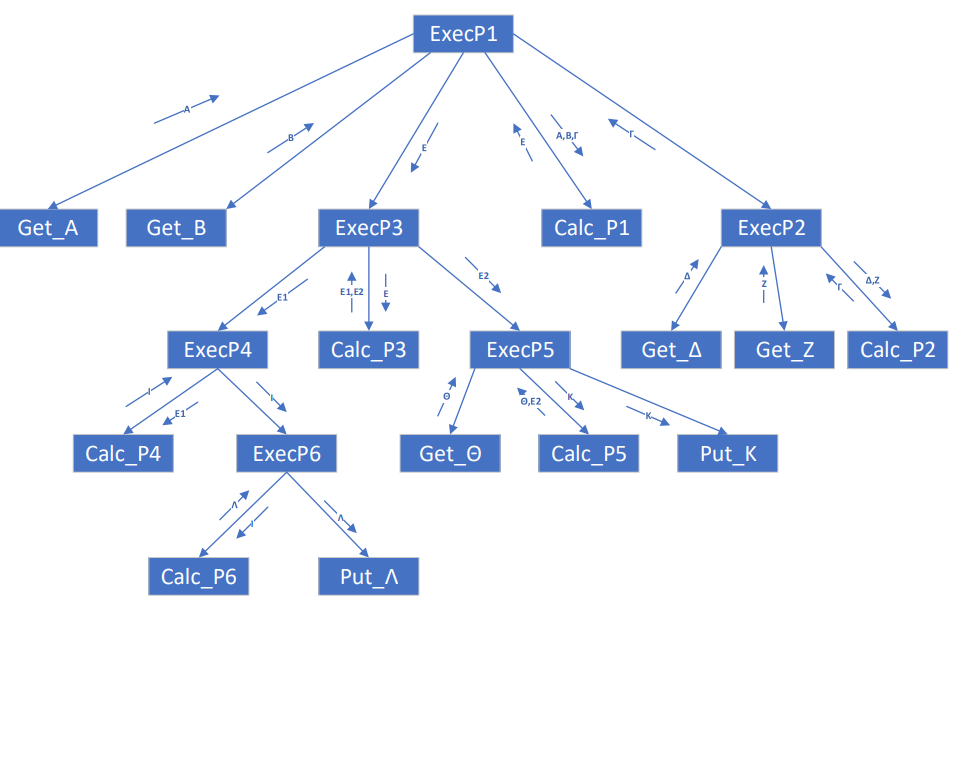
\includegraphics[scale=0.5]{MerosG/DDP}
\end{tabular}
\end{center}

\newpage
\item Τμηματα Ψευδοκωδικα:
\begin{enumerate}[label*=\roman*]
	\item Mονάδα ελέγχου του μετασχηματισμού Ρ1
	
	\begin{lstlisting}
	$Procedure$ $ExecP1$
		$Local$ $var$ A,B,G,E
		$Arxikopoihse$ A,B,G,E
		$Call$ $Get\_A(A)$
		$Call$ $Get\_B(B)$
		$Call$ $Calc\_P1($A,B,G,E$)$
		$Call$ $ExecP3(E)$
	$End\_Procedure$
	\end{lstlisting}
	
	\item  Μονάδα υπολογισμού του μετασχηματισμού Ρ2
	\begin{lstlisting}
	$Procedure$ $Calc\_P2($D$,$Z$:IN,$G$:IN/OUT)$
		...
		$Upologise$ G
		...
	$End\_Procedure$
	\end{lstlisting}
	
	\item Μονάδα παρουσίασης του μετασχηματισμού Ρ5
	\begin{lstlisting}
	$Procedure$ $Put\_K(K:IN)$
		...
		$Grapse$ K
		...
	$End\_Procedure$
	\end{lstlisting}
	
	\item Μονάδα διαχείρισης δεδομένων του μετασχηματισμού Ρ1
	\begin{lstlisting}
	$Procedure$ $Get\_B(B:IN/OUT)$
		...
		$Diavase$ B
		...
	$End\_Procedure$
	\end{lstlisting}
\end{enumerate}
\end{enumerate}

\end{document}